%%%%%%%%%%%%%%%%%%%%%%%%%%%%%%%%%%%%%%%%%%%%%%%%%%%%%%%%%%%%%%%%%%%%%%%%%
%                                                                       %
% ustthesis_test.tex: A template file for usage with ustthesis.cls      %
%                                                                       %
%%%%%%%%%%%%%%%%%%%%%%%%%%%%%%%%%%%%%%%%%%%%%%%%%%%%%%%%%%%%%%%%%%%%%%%%%

\documentclass{ustthesis}

% \usepackage{mathpazo,
\usepackage{amsmath, amssymb}
% epsfig,enumerate,bbm,calc,color,ifthen,capt-of} % original was times, but I think it's ugly; we use the same as IEEE CompSoc
\usepackage{algorithm}
% \usepackage[noend]{algorithmic}
\usepackage{algorithmic}
% \usepackage[center]{subfigure}
\usepackage{color,graphicx}
\usepackage{siunitx}
\usepackage{soul}
\usepackage{graphics} % for pdf, bitmapped graphics files
\usepackage{subcaption}
\newtheorem{proof}{Proof}
\usepackage{bookmark}
\usepackage{hyperref} % for better viewing experience  -- added by alan
\usepackage{textcomp}
\usepackage{multirow}
\usepackage{nth}
\usepackage{indentfirst}
\usepackage{siunitx}
\usepackage{changepage}
% \usepackage{setspace}
% \usepackage[a4paper, margin=25mm]{geometry}
\usepackage[a4paper, margin=25mm,textheight=247mm,textwidth=145mm]{geometry}

% Alan: begin the font trial
% Euler for math | Palatino for rm | Helvetica for ss | Courier for tt
% \renewcommand{\rmdefault}{ppl} % rm

% Lei: rouphly 32 lines for 12pt font size and 1.5 line spacing
\linespread{1.05}

% \usepackage[scaled]{helvet} % ss
% \usepackage{courier} % tt
%\usepackage{euler} % math
% \usepackage{eulervm} % a better implementation of the euler package (not in gwTeX)
% \normalfont
% \usepackage[T1]{fontenc}
% Alan: end the font trial


\DeclareMathOperator*{\argmax}{\arg\!\max}
\DeclareMathOperator*{\argmin}{\arg\!\min}

\newcommand{\red}[1]{#1}
\newcommand{\tab}[1]{\hspace{3mm}}

\newcommand{\bx}{\mathbf{x}}
\newcommand{\bX}{\mathbf{X}}
\newcommand{\by}{\mathbf{y}}
\newcommand{\bY}{\mathbf{Y}}
\newcommand{\bD}{\mathbf{D}}
\newcommand{\bE}{\mathbf{E}}
\newcommand{\ba}{\mathbf{a}}
\newcommand{\bs}{\mathbf{s}}
\newcommand{\bn}{\mathbf{n}}
\newcommand{\bI}{\mathbf{I}}
\newcommand{\bsigma}{\mathbf{\sigma}}
\newcommand{\cS}{\mathcal{S}}
\newcommand{\cX}{\mathcal{X}}
\newcommand{\cA}{\mathcal{A}}
\newcommand{\cB}{\mathcal{B}}
\newcommand{\cD}{\mathcal{D}}
\newcommand{\bu}{\mathbf{u}}
\newcommand{\bv}{\mathbf{v}}
\newcommand{\ts}{\textsuperscript}
\newcommand{\etal}{{\em et al.}}
\newcommand{\norm}[1]{\left\lVert#1\right\rVert}
\DeclareMathOperator{\atantwo}{atan2}
\newcommand{\argminE}{\mathop{\mathrm{argmin}}}
% \newcommand\thelinespace{\expandafter\string\the\baselinestretch}
\setcounter{tocdepth}{3}
\setcounter{secnumdepth}{3}

% \renewcommand{\familydefault}{\rmdefault}

% \usepackage{latexsym}
    % Use the "latexsym" package when encountering the following error:
    %   ! LaTeX Error: Command \??? not provided in base LaTeX2e.
% \usepackage{epsf}
    % Use the "epsf" package for including EPS files.

%%%%%%%%%%%%%%%%%%%%%%%%%%%%%%%%%%%%%%%%%%%%%%%%%%%%%%%%%%%%%%%%%%%%%%%%%
%                                                                       %
% Preambles. DO NOT ERASE THEM. Change to suite your particular purpose.%
%                                                                       %
%%%%%%%%%%%%%%%%%%%%%%%%%%%%%%%%%%%%%%%%%%%%%%%%%%%%%%%%%%%%%%%%%%%%%%%%%

\title{Sample Title for HKUST Thesis}  % Title of the thesis.
\author{Ming~XIAO}     % Author of the thesis.

% NOTE: choose your degree
\degree{\MPhil}             % Degree for which the thesis is.
% %% or
% \degree{\PhD}              % Degree for which the thesis is.

\department{Electronic and Computer Engineering}       % Department to which the thesis

\advisor{Prof.~Lei~LI}     % Supervisor.

% NOTE: Uncomment this line if you have a co-supervisor
% \coadvisor{Prof.~Mazi~Zhang}     % Co Supervisor.

\depthead{Prof.~Meimei~Han}    % department head.

\defencedate{2019}{08}{05}      % \defencedate{year}{month}{day}.

% NOTE:
%   According to the sample shown in the guidelines, page number is
%   placed below the bottom margin.  However, if the author prefers
%   the page number to be printed above the bottom margin, please
%   activate the following command.
% \PNumberAboveBottomMargin

\graphicspath{{./figure/}}
\begin{document}

%%%%%%%%%%%%%%%%%%%%%%%%%%%%%%%%%%%%%%%%%%%%%%%%%%%%%%%%%%%%%%%%%%%%%%%%%
%                                                                       %
% Now the actual Thesis. The order of output MUST be followed:          %
%                                                                       %
%    1) TITLEPAGE                                                       %
%                                                                       %
% The \maketitle command generates the Title page as well as the        %
% Signature page.                                                       %
%                                                                       %
%%%%%%%%%%%%%%%%%%%%%%%%%%%%%%%%%%%%%%%%%%%%%%%%%%%%%%%%%%%%%%%%%%%%%%%%%
\maketitle

%%%%%%%%%%%%%%%%%%%%%%%%%%%%%%%%%%%%%%%%%%%%%%%%%%%%%%%%%%%%%%%%%%%%%%%%%
%                                                                       %
%     2) DEDICATION (Optional)                                          %
%                                                                       %
% The \dedication and \enddedication commands are optional. If          %
% specified it generates a page for dedication.                         %
%
%%%%%%%%%%%%%%%%%%%%%%%%%%%%%%%%%%%%%%%%%%%%%%%%%%%%%%%%%%%%%%%%%%%%%%%%%

% \dedication
% This is an optional section.
% \enddedication

%%%%%%%%%%%%%%%%%%%%%%%%%%%%%%%%%%%%%%%%%%%%%%%%%%%%%%%%%%%%%%%%%%%%%%%%%
%                                                                       %
%     3) SIGNATURE                                                      %
%                                                                       %
% \signature and \endsignature defines the                              %
% signature page of the Thesis especially for ece.                      %
%                                                                       %
%%%%%%%%%%%%%%%%%%%%%%%%%%%%%%%%%%%%%%%%%%%%%%%%%%%%%%%%%%%%%%%%%%%%%%%%%

\signature
		\begin{figure}[!hb]
		\begin{tabular}{ll}
		Thesis Examination Committee &  \\[8pt]
		1. Prof. Lei LI (Supervisor)   &  Department of Electronic and Computer Engineering \\[8pt]
		2. Prof. xxx              &  Department of Electronic and Computer Engineering \\[8pt]
		3. Prof. xxx               &  Department of Electronic and Computer Engineering \\[8pt]
		4. Prof. xxx               &  Department of Mathematics\\[8pt]
		5. Prof. xxx (External Examiner)  & Department of Electrical Engineering\\[8pt]
		                                   &  Vienna University of Technology \\[8pt]
    % NOTE LEI:
    %   In case the space is not enough, try \footnotesize for this part.
		% \footnotesize{Thesis Examination Committee} &  \\[8pt]
		% \footnotesize{1. Prof. xxx (Supervisor)}   &  \footnotesize{Department of Electronic and Computer Engineering} \\[8pt]
		% \footnotesize{2. Prof. xxx}   &  \footnotesize{Department of Electronic and Computer Engineering} \\[8pt]
		% \footnotesize{3. Prof. xxx}   &  \footnotesize{Department of Electronic and Computer Engineering} \\[8pt]
		% \footnotesize{4. Prof. xxx}            &  \footnotesize{Department of Mathematics }\\[8pt]
		% \footnotesize{5. Prof. xxx (External Examiner)}  & \footnotesize{Department of Electrical Engineering and} \\[8pt]
		%                               & \footnotesize{Information Technology} \\[8pt]
		%                               &  \footnotesize{Vienna University of Technology} \\[8pt]
		\end{tabular}
		\end{figure}
\endsignature

%%%%%%%%%%%%%%%%%%%%%%%%%%%%%%%%%%%%%%%%%%%%%%%%%%%%%%%%%%%%%%%%%%%%%%%%%
%                                                                       %
%     3) ACKNOWLEDGMENTS                                                %
%                                                                       %
% \acknowledgments and \endacknowledgments defines the                  %
% Acknowledgments of the author of the Thesis.                          %
%                                                                       %
%%%%%%%%%%%%%%%%%%%%%%%%%%%%%%%%%%%%%%%%%%%%%%%%%%%%%%%%%%%%%%%%%%%%%%%%%

\acknowledgments

First of all, I am truly grateful for being one of the first PhD students supervised by Prof. Li.
He was full of passion and patience when helping me build the know-how for this degree. It has been a great pleasure for me to be part of this team and grow together with the lab during the last four years. Furthermore, I would like to thank all of the members of the thesis examination committee for their careful examination of my thesis.

Finally, I would not stand at this current point without their endless love and unconditional support for all these years.

\endacknowledgments

%%%%%%%%%%%%%%%%%%%%%%%%%%%%%%%%%%%%%%%%%%%%%%%%%%%%%%%%%%%%%%%%%%%%%%%%%
%                                                                       %
%     4) TABLE OF CONTENTS                                              %
%                                                                       %
%%%%%%%%%%%%%%%%%%%%%%%%%%%%%%%%%%%%%%%%%%%%%%%%%%%%%%%%%%%%%%%%%%%%%%%%%

\tableofcontents

%%%%%%%%%%%%%%%%%%%%%%%%%%%%%%%%%%%%%%%%%%%%%%%%%%%%%%%%%%%%%%%%%%%%%%%%%
%                                                                       %
%     5) LIST OF FIGURES (If Any)                                       %
%                                                                       %
%%%%%%%%%%%%%%%%%%%%%%%%%%%%%%%%%%%%%%%%%%%%%%%%%%%%%%%%%%%%%%%%%%%%%%%%%

\listoffigures

%%%%%%%%%%%%%%%%%%%%%%%%%%%%%%%%%%%%%%%%%%%%%%%%%%%%%%%%%%%%%%%%%%%%%%%%%
%                                                                       %
%     6) LIST OF TABLES (If Any)
%                                                                       %
%%%%%%%%%%%%%%%%%%%%%%%%%%%%%%%%%%%%%%%%%%%%%%%%%%%%%%%%%%%%%%%%%%%%%%%%%

\listoftables

%%%%%%%%%%%%%%%%%%%%%%%%%%%%%%%%%%%%%%%%%%%%%%%%%%%%%%%%%%%%%%%%%%%%%%%%%
%                                                                       %
%     7) ABSTRACT                                                       %
%                                                                       %
% \abstract and \endabstract are used to define a short Abstract for    %
% the Thesis.                                                           %
%                                                                       %
%%%%%%%%%%%%%%%%%%%%%%%%%%%%%%%%%%%%%%%%%%%%%%%%%%%%%%%%%%%%%%%%%%%%%%%%%

\begin{abstract}

  Compared to known and static environments, mobile robot navigation within dynamic, pedestrian-rich and unfamiliar environments is still challenging. To model these scenarios through traditional hand-crafted features is not efficient and effective enough. Deep learning has achieved state-of-the-art results in various fields of study, especially in complex task modelling, in the last several years.
  Sensorimotor learning has also shown great potential to solve many complicated manipulation tasks. However, the potential exploration of deep learning in robot sensorimotor policies, especially for mobile robot navigation is still limited.

  % Additionally, practical applications of traditional robot control and the policy search pipeline often require hand-engineered components for perception, state estimation, and low-level control. For example, in robot navigation, a geometrical map needs to be predefined. After that, the path and trajectory are planned on the map. Finally, the robot outputs the related actions to actuators based on low-level controllers.
  % Traditionally, consistently optimizing the uncertainties generated from each part is unrealistic. Deep learning, especially deep reinforcement learning and imitation learning, provide possible solutions for this problem.

  In this thesis, we are targeting to leverage fully differentiable structures to realize end-to-end sensorimotor learning for ground mobile robot navigation. We aim to answer the following questions:
  (1) How do we learn the sensorimotor policy for mobile robot navigation? And (2) how should we deploy it in the real world considering the reality gap and uncertainties? For question (1), we proposed two structures for sensorimotor learning through both deep reinforcement learning and inverse imitation learning. For the second question, we propose \textit{shift loss} to constraint the sequence input domain adaptation and combine it with a generative adversarial network to translate the real-world image streams back to the synthetic domain during the deployment phase. The uncertainties of deep learning are also considered to learn a stochastic policy. By conducting a series of experiments, both in simulated and real-world environments, we show how these learned sensorimotor models can be successfully applied in both indoor and outdoor mobile robot navigation scenarios.

\end{abstract}


%%%%%%%%%%%%%%%%%%%%%%%%%%%%%%%%%%%%%%%%%%%%%%%%%%%%%%%%%%%%%%%%%%%%%%%%%
%                                                                       %
%     8) The Actual Contents                                            %
%                                                                       %
% The command \chapters MUST BE USED to ensure that the entire content  %
% of the Thesis is double-spaced (in version 1.0).                      %
%                                                                       %
% However, in version 2.0, \chapters will be automatically added in     %
% the beginning of the first chapter.                                   %
%                                                                       %
%%%%%%%%%%%%%%%%%%%%%%%%%%%%%%%%%%%%%%%%%%%%%%%%%%%%%%%%%%%%%%%%%%%%%%%%%

%%\chapters         % Not necessary with ustthesis.cls (v2.0).

%%%%%%%%%%%%%%%%%%%%%%%%%%%%%%%%%%%%%%%%%%%%%%%%%%%%%%%%%%%%%%%%%%%%%%%%%
%                                                                       %
% Each chapter is defined via the \chapter command. The usual sectional %
% commands of LaTeX are also available.                                 %
%                                                                       %
%%%%%%%%%%%%%%%%%%%%%%%%%%%%%%%%%%%%%%%%%%%%%%%%%%%%%%%%%%%%%%%%%%%%%%%%%



\chapter{Introduction}
\label{ch:intro}


Intelligent robots are influencing many aspects of the world nowadays, from collaborative robot arms in factories to L4 autonomous driving technology, from biped household robots to quadruped mobile military agents, and from unmanned surface vehicles to quadrotor swarms. The more deeply we imagine the future, the more indispensable we find robot services.

For mobile robots, navigation is always the kernel function. However, compared with the automation of manipulation, mobile robot navigation is evolving more slowly. In the classical manipulation and manufacturing scenarios, the workspace of robots is usually well defined, and the robots can perform correctly under human-designed programming, without any interaction between uncertain objects and themselves. If we regard \textit{replacing the repetitive workloads} as the first step, we should start to consider \textit{living with the robot} in the next step. For mobile robots, to be incorporated into human's daily life, they must be intelligent in unknown and pedestrian-rich environments for tasks like autonomous driving, cargo delivers and household mobile robots, which is \textit{behaving like a human}.

Human beings can navigate in crowded environments smartly without dependence on pre-defined high-resolution maps. We can also explore unknown environments without taking time to think about the information gain or frontiers. To navigate safely and efficiently like a human being, mobile robots should be able to perceive and predict behaviours of unfamiliar and dynamic agents. Based on the implicit or explicit understanding, an accessible policy considering various constraints is needed to guide the robots.


Deep learning, as a solution for artificial intelligence, is capable of building progressively meaningful feature abstraction of input data.
It plays an essential role in various fields of study \cite{Goodfellow-et-al-2016}, bringing the state of the art in image classification \cite{he2016deep,huang2017densely, krizhevsky2012imagenet},
semantic segmentation \cite{chen2016deeplab, long2015fully},
human-level game playing \cite{mnih2016asynchronous, mnih2015human}, driving real robotic systems in navigation \cite{tai2017virtual, zhang2017deep, zhu2017target}
and manipulation \cite{levine2016end,yu2018one} tasks.

We may be witnessing the most rapidly growing trend of deep learning techniques for robotics tasks in recent years.
Replacing hand-crafted features with learned hierarchical distributed deep features, and learning control policies directly from high-dimensional sensory inputs, the robotics community is making substantial progress towards building fully autonomous intelligent systems.

% \section{Deep Learning for Robotics: From Perception to Control}
Autonomous intelligent robotics systems require two essential building blocks: perception and control.

The perception pipeline can be viewed as a passive procedure:
intelligent agents receive observations from the environment,
then infer desired properties or detect target quantities from those sensory inputs.
We refer readers to \cite{deng2014tutorial} and \cite{guo2016deep} for a comprehensive overview of deep learning techniques for perception.
Compared with pure perception, the problem of control for autonomous agents goes one step further,
seeking to actively interact with or influence the environment by conducting sequences of actions.
This active nature leads to the following major distinctions between perception and control, in terms of deep-learning-based approaches:

\textbf{Data distribution:} When learning perception through supervised learning techniques,
the training datasets are collected and labelled before the learning phase begins.
In this case, the data points can be viewed as being independently and identically distributed (i.i.d),
such that a direct mapping from the input to the labels can be learned via standard stochastic gradient descent methods and variants.
In contrast, for control, the datasets are collected in an on-line manner, which makes the data points sequential in nature: the consecutive observations received by the agent are temporally correlated since the agent actively influences the data distribution by the actions it takes. Ignoring this underlying temporal correlation would lead to compounding errors \cite{bagnell2015invitation}.

\textbf{Supervision signal:} The supervision for learning perception is often direct and strong,
in that each training sample is provided along with its ground truth label.
In control tasks, on the other hand, either only sparse reward signals are available when learning behaviors through \textit{deep reinforcement learning} and \textit{inverse reinforcement learning},
or the feedback is often delayed and not instantaneous,
even when demonstrations from experts are provided in the scenario of \textit{imitation learning},
since the credit for achieving a certain goal needs to be correctly assigned to all the actions taken along the trajectory.

\textbf{Data collection:} As discussed before, the dataset for perception can be collected off-line, while the dataset for control has to be collected in an on-line manner, since actions are actively involved in the learning process. This greatly limits the number of samples one can collect, since executing actions in the real world with real robotics systems is a relatively expensive procedure. In cases where the control policies are trained in simulation, the problem of the \textit{reality gap} arises when they are deployed in real-world scenarios, where the discrepancies between the modalities of the synthetic renderings and the real sensory readings impose major challenges.

% \section{Sensorimotor Learning}
\label{sec:lb_sensorimotor}

Following the discussion above, the sensorimotor learning problem targets mapping raw sensor information to the actuator commands directly, for both manipulation and navigation tasks mainly through \textit{deep reinforcement learning}. A typical reinforcement learning pipeline is shown in Fig. \ref{fig:rlloop}

\begin{figure}[!ht]
   \centering
   \includegraphics[width=0.65\columnwidth]{intro_figs/rlloop}
    \caption{The typical reinforcement learning loop for robotics tasks.
    The agent takes the action $\ba_{t}$ in state $\bs_{t}$, receives a reward $R_{t+1}$, and evolves to the next state $\bs_{t+1}$.}
   \label{fig:rlloop}
\end{figure}

In terms of manipulation, the tasks being considered for evaluating Deep Reinforcement Learning (DRL) algorithms are more standardized in the recent literature \cite{heess2017emergence,lillicrap2015continuous,mnih2016asynchronous,schulman2015trust,wu2017scalable}.
Most such works benchmark the proposed algorithms on standard tasks,
including \textit{reaching}, \textit{pushing}, \textit{pick-and-place}, etc.,
using the \textit{MuJoCo} simulator \cite{todorov2012mujoco}.
Below we focus on the works that are presented with real robotic experiments.

An asynchronous version of NAF is proposed in \cite{gu2016deep}.
Taking in the low dimensional states as inputs (joint angles, end-effector poses, as well as their time derivatives, and the pose of the target),
in addition to well-shaped reward signals, it allows the robot to learn a real-world door opening task in about $2.5$ hours in a completely end-to-end manner,
achieving a $100\%$ success rate.

Model-based approaches like guided policy search (GPS)\cite{levine2016end} can also successfully train deep visuomotor policies.
Their proposed visuomotor policy network takes as input monocular RGB images and passes them through several convolutional layers and a spatial soft argmax layer,
which are then concatenated with the robot configurations (joint angles, end-effector poses).
These representations are then passed through several fully connected layers and used to predict the corresponding motor torques.
Various experiments on a \textit{PR2} robot (with a $7$-DOF arm)
such as hanging a coat hanger on a clothes rack,
inserting a block into a shape sorting cube,
or screwing on a bottle cap have been demonstrated to validate the effectiveness of the approach.
This method, however, requires a known and fully observed state space,
which could limit its potential use cases.

Model-based DRL methods are also utilized by
\cite{finn2016deep} and \cite{tzeng2015towards},
learning useful state representations for generating successful control policies.
\cite{fu2016one} proposed one-shot learning of manipulation skills through model-based reinforcement learning by leveraging the neural network priors as a dynamic model.
Learning dexterous manipulation skills with multi-fingered hands,
for which model-based \cite{gupta2016learning, kumar2016optimal} and model-free \cite{popov2017data} DRL algorithms have been proposed and demonstrated in real robotic experiments,
is quite challenging.

While many works have carefully designed their reward structure to guide reinforcement learning,
some research \cite{martin2018learning} tried to speed up learning from only binary or sparse rewards,
under the observation that well-shaped rewards can often bias the learned control policy into potentially suboptimal directions.
In contrast, when only sparse reward signals are provided to the agent, the learner can discover novel and potentially preferable solutions.
To achieve this, alongside the policy learning for the main task, it learns policies (which they refer to as intentions) for a set of semantically grounded auxiliary tasks,
whose supervision signals can be easily obtained by the activation of certain sensors.
Then a scheduling policy is learned to sequence the intention-policies.
Their proposed algorithm is able to learn to solve challenging manipulation tasks from scratch,
such as stacking two blocks into a tower or cleaning up a desk by putting objects into a box with a lid that can be opened,
with a $9$-DOF robot arm. Moreover, in their real-world experiments, a single robot arm learns a lifting task in about $10$ hours.

Our work focuses on the robot navigation problem.
Autonomous navigation is one of the essential problems and challenges in mobile robotics.
It can roughly be described as the ability of a robot to plan and follow a trajectory through the environment to reach a certain goal location without colliding with any obstacles in between.
The recent literature has seen a growing number of methods proposed to tackle the task of autonomous navigation with DRL algorithms.
These works formulate the navigation problem as MDPs or POMDPs that first take in the sensor readings (colour/depth images, laser scans, etc.) as observations and stack or augment them into states,
and then search for the optimal policy that is capable of guiding the agent to navigate to goal locations in a timely and collision-free manner.
Below we discuss several representative works in this category that target the field of robotics.

Zhu \textit{et al.} \cite{zhu2017target} input both the first-person view and the image of the target object to the A3C model,
formulating a target-driven navigation problem based on the universal value function approximators \cite{schaul2015universal}.
The training of their model requires the output of the feature from a pre-trained \textit{ResNet}-$50$ \cite{he2016deep} and is performed in an indoor simulator \cite{kolve2017ai2}
where each new room is regarded as a new scene for which several scene-specific layers are added as another output head of the model.
The success rate for generalizing the navigation policies to new targets one step away from the trained targets is $70\%$,
and around $42\%$ for those that are two steps away.
For navigation tasks with optimal solutions of $17.6$ steps,
it achieves a $210.7$ average trajectory length after being trained on $100$ million frames with an A3C agent.
The trained policy was able to navigate a real robot inside an office environment after being fine-tuned on images collected from the real scene.

Zhang \textit{et al.} \cite{zhang2017deep} worked on a deep \textit{successor representation} formulation \cite{barreto2017successor, kulkarni2016deep} for the $Q$-value function,
targeting learning representations that are transferrable between related navigation tasks.
Following the observation that most of the \textit{value-based} DRL methods, such as DQN,
usually learn a black-box function approximator for the optimal value functions,
which makes how to transfer the knowledge gained from one task to a related task unclear,
they extended the \textit{successor feature representation} that decouples the learning of the optimal value functions into two parts,
learning task-specific reward functions, and learning task-specific features, and how those features evolve under the current task dynamics.
While this representation has been shown to work well on transferring learned policies to differently scaled reward functions and changed goals in fixed environments,
Zhang \textit{et al.} \cite{zhang2017deep} extended the formulation to cope with transferring policies to new environments.

% \section{Contributions}
% % \subsection{Markov Decision Process}
% We formalize a robotics task (e.g., navigation, manipulation) as a \textit{Markov Decision Process} (MDP), in which the agent interacts with the environment through a sequence of observations, actions, and reward signals. An MDP is a $5-$tuple $\left< \mathcal{S}, \mathcal{A}, P, \mathcal{R}, \gamma \right>$:
% $\mathcal{S}$: set of all states.
% $\mathcal{A}$: set of all actions.
%   %\item $\mathcal{P}(\bs_{t+1}|\bs_{t}, \ba_{t})$: defines the probability of transisting to state $\bs_{t+1}$ from a state-action pair $(\bs_{t}, \ba_{t})$.
%   %\item $\mathcal{P}(S_{t+1}|S_{t}, A_{t})$: defines the probability of transisting to a next state from a state-action pair.
% $\mathcal{P}$: the transition dynamics,
% where $P(\bs'|\bs, \ba)$ defines the distribution of the next state $\bs'$ by taking action $\ba$ in state $\bs$,
% where $\bs,\bs'\in\mathcal{S}, \ba\in\mathcal{A}$. We also denote the initial state distribution $P(\bs_0)$ as $\rho_0$.
%   %\item $\mathcal{R}(\bs_{t}, \ba_{t})$: defines the instantaneous scalar reward received by the agent from a state-action pair $(\bs_{t}, \ba_{t})$.
%   %\item $\mathcal{R}(S_{t}, A_{t})$: defines the instantaneous scalar reward received by the agent from a state-action pair.
%   % \item $\mathcal{R}(\bs_t,\ba_t,\bs_{t+1})$ \hl{check again here}: defines the instantaneous scalar reward received by the agent from a state-action pair. Usually one is interested in the expected reward achieved with a state-action pair: $R_{t+1}(\bs_t,\ba_t)=\mathbf{E}_{\bs_{t+1}\sim\mathcal{P}(\cdot|\bs_t,\ba_t)}\left[\mathcal{R}(\bs_t,\ba_t,\bs_{t+1})\right]$; in the following descriptions, we mostly use $R_{t+1}$ to be short for $R_{t+1}(\bs_t,\ba_t)$.
% $\mathcal{R}$: set of all possible rewards.
%   In the following, we denote the instantaneous scalar reward received by the agent by taking action $\ba_t$ from state $\bs_t$ as $R_{t+1}(\bs_t,\ba_t)$,
%   and use $R_{t+1}$ as short for $R_{t+1}(\bs_t,\ba_t)$.
%   There also exist other definitions of the reward function that depend only on the state itself,
%   in which $R(\bs)$ refers to the reward signal that the agent receives by arriving at state $\bs$.
%   In some of the following discussions, the negative counterpart of the reward function,
%   the cost function, is used, and is denoted as $c(\bs)$.
% $\gamma$: a discount factor in the range of $[0,1]$.
%
% In an MDP, the agent takes an action $\ba_{t}$ in state $\bs_{t}$, receives a reward $R_{t+1}$, and transits to the next state $\bs_{t+1}$ following the transition dynamics $\mathcal{P}(\bs_{t+1}|\bs_{t},\ba_{t})$.
%
% In robotics, we mainly consider \textit{episodic} MDPs, where there exists a \textit{terminal state} (e.g., a mobile ground vehicle reaches a certain goal location, a manipulator successfully grabs a red cup) that, once reached, terminates the current \textit{episode}. Also for an \textit{episodic} MDP with a time horizon of $T$, an \textit{episode} will still be terminated after a maximum of $T$ time steps, even if by then the \textit{terminal state} has not yet been reached.
%
% Another point worth mentioning is the \textit{partial observability}.
% In a robotics task, an autonomous agent perceives the world with its onboard sensor (e.g., RGB/depth camera, IMU, laser range sensor, 3D Lidar),
% receiving one observation
% %$\mathbf{x}_{t}$ (e.g., one color/depth image, one laser scan, one ... point cloud)
% per time step. However, simply representing $\bs_{t}$ by $\mathbf{x}_{t}$ often does not satisfy the \textit{Markov} property: one such sensor reading can hardly capture all the necessary information for the agent to make decisions in the future,
% in which case the underlying procedure is called a Partial Observeble MDP (POMDP).
% This is often dealt with by either stacking several (e.g, $N$) consecutive observations $\{ \mathbf{x}_{t-N+1}, \mathbf{x}_{t-N+2}, \dots, \mathbf{x}_{t} \}$ to represent $\bs_{t}$, or by feeding $\mathbf{x}_{t}$ into a \textit{recurrent} neural network instead of a \textit{feed forward} one,
% such that the past information is naturally accounted with (e.g., by the cell state when using the long short-term memories (LSTMs).
%
% Reinforcement learning agents are designed to learn from interactions how to behave to achieve a certain goal \cite{sutton1998reinforcement}.
% More precisely, here the objective of learning is to maximize the \textit{expected discounted return},
% where the \textit{discounted return} is defined as follows:
% \begin{align}
%   G_{t}
% &=
%   R_{t+1} + \gamma R_{t+2} + \gamma^2 R_{t+3} + \dots + \gamma^{T-t-1} R_{T}
% \\&=
%   \sum_{k=t}^{T} \gamma^{k-t} R_{k+1}.
% \end{align}
%
% To learnin sensorimotor, two important definitions are introduced:
% \begin{itemize}
%   \item \textbf{Policies}: $\pi, \mu$
%     \begin{itemize}
%       \item $\pi(\ba|\bs)$: stochastic policy, where actions are drawn from a probability distribution defined by $\pi(\ba|\bs)$.
%       \item $\mu(\bs)$: determinstic policy, where actions are deterministically selected for a given state $\bs$.
%     \end{itemize}
%   \item \textbf{Value functions}: $V, Q$
%     \begin{itemize}
%       \item $V^{\pi}(\bs)$: state-value function, defined as the expected return when starting from state $\bs$ and following policy $\pi$ thereafter: % estimates how good it is to be in a particular state $\bs$ following policy $\pi$
%       \begin{align}
%         V^{\pi}(\bs)
%       &=
%         \mathbb{E}_{\pi}\left[ G_t | \bs_t=\bs \right]
%       \\&=
%         \mathbb{E}_{\pi}\left[ \sum_{k=t}^{T}\gamma^{k-t} R_{k+1} | \bs_t=\bs \right].
%         \label{equ:value-reward}
%       \end{align}
%       \item $Q^{\pi}(\bs, \ba)$: action-value function,
%       defined as the expected return by taking the action $\ba$ from state $\bs$,
%       then following $\pi$ thereafter: % estimates how good it is to take a particular action $\ba$ in a particular state $\bs$ following policy $\pi$
%       \begin{align}
%         Q^{\pi}(\bs,\ba)
%       &=
%         \mathbb{E}_{\pi}\left[ G_t | \bs_t=\bs, \ba_t=\ba \right]
%       \\&=
%         \mathbb{E}_{\pi}\left[ \sum_{k=t}^{T}\gamma^{k-t} R_{k+1} | \bs_t=\bs, \ba_t=\ba \right].
%         \label{equ:q-reward}
%       \end{align}
%       \item $Q^{*}(\bs, \ba)$: optimal value function (We omit the case for state-value function $V$ here since the action-value function $Q$ is a much more effective representation for control.):
%       \begin{align}
% %        V_{*}(\bs)
% %      &=
% %        \max_{\pi} V_{\pi}(\bs)
% %      \\
%         Q^{*}(\bs,\ba)
%       &=
%         \max_{\pi} Q^{\pi}(\bs,\ba).
%       \end{align}
%       \item $\pi^{*}(\ba|\bs)$: optimal policy:
%       \begin{align}
%         \pi^{*}(\ba|\bs)
%       &=
%         {\argmax}_{\ba} Q^{*}(\bs,\ba).
%       \end{align}
%     \end{itemize}
% \end{itemize}

%%%%%%%%%%%%%%%%%%%%%%%  contributions  %%%%%%%%%%%%%%%%%%%%%%%%
The contributions of this thesis are as follows:
\begin{itemize}
  \item In Chapter \ref{ch:intro}, we discuss the evolution of learning-based methods on robotics. Compared with pure supervised learning, robotics tasks are normally defined as deep reinforcement learning or inverse imitation learning. We summarised the same discussions in \cite{tai2016survey} before.
  \item In Chapter \ref{ch:obstacle}, we propose active obstacle avoidance through deep reinforcement learning. Even though the network is initialized by weights trained from supervised learning, the online learning process of reinforcement learning encourages the model to explore more robust feature patterns in the network. This works was previously presented in \cite{tl_rcar_2016} and \cite{tai2016towards}.
  \item In Chapter \ref{ch:mfrl}, we consider model-free reinforcement learning to tackle the mapless navigation of mobile robots. The robot successfully navigates to various targets in an indoor environment based on local lidar sensor information and coarse target guidance. This work was published previously as \cite{tai2017virtual}.
  \item In Chapter \ref{ch:il}, we consider GAN-style imitation learning to learn complex socially compliant navigation behaviours among pedestrians. This work was described previously in \cite{tai2018social}.
  \item In Chapter \ref{ch:vrg}, we propose a new shift loss, which enables generating consistent synthetic image streams without imposing temporal constraints, or even sequential training data. Additionally, since we decouple the policy training and the adaptation operations, the preparations for transferring the polices from simulation to the real world can be conducted in parallel with the training of the control policies. This work was previously published as \cite{zhang2019vrgoggles}.
  \item In Chapter \ref{ch:uail}, we follow the recent real-to-sim pipeline by translating a testing world image back to the training domain when using a trained policy. In the translation process, a stochastic generator is used to generate various images stylized under the training domain randomly or directionally. Through the uncertainty-aware imitation learning policy, we can easily choose the safest policy with the lowest uncertainty among the generated images. This work was presented before as \cite{tai2019end}.
\end{itemize}



% NOTE Lei:
%    Normally we don't need part, but I used it in my thesis
\part{From Supervisd Learning to Reinforcment Learning}
\label{part1}
\chapter{Active Obstacle Avoidance Learning}
\label{ch:obstacle}

%###########################################################
%---------------------------------introduction--------------------------

\section{Introduction}

\subsection{Motivation}
\label{sec:ob_motivation}
Obstacle avoidance is fundamental for mobile robots in divers tasks, like cleaning, mining, and rescue, etc.
In this chapter, we deal with a classic task for a mobile robot equipped with a depth sensor: attempting to avoid collisions with obstacles while navigating in an unknown environment.
Using stereo vision systems or radar sensors as aids, researchers often build the geometry or topological mapping of environments \cite{liu2015incremental, liu2012markov} to make navigation decisions based on a global representation. Such methods regard the environment as a geometrical world and decisions are only made with preliminary features without an online learning process. Specific logic has to be particularly designed for different environments. It is still a challenge for mobile robots to rapidly adapt to a new environment. Active learning for mobile robots to achieve tasks have been widely achieved for mobile robot navigation tasks like localisation \cite{burgard1997active, singh2018active}. In this chapter, we aim for robots to actively learn essential features for obstacle avoidance.

Convolutional neural network (CNN), a typical model for deep-learning and cognitive recognition, are the state-of-the-art in computer vision tasks. The Success of type of hierarchical model also motivates robotics scientists to apply deep learning algorithms in common robotics problems like recognition and obstacle avoidance \cite{giusti2016machine, muller2005off, tai2016deep}.

As with most supervised learning algorithms, CNN extracts feature representations through training with a massive amount of labelled samples.
However, unlike typical computer vision tasks, robot navigation usually happens in dynamic environments with high probability and uncertainty. The overfitting problem of supervised learning limits the perception ability of hierarchical models for unseen inputs, and it is unrealistic for mobile robots to collect datasets covering all of the possible conditions. Besides this, the time-consuming work of dataset collection and labelling seriously influences the application of CNN-based learning methods. Another common problem is that robotics research usually considers the CNN mechanism as a black box. There lacks a proper metric to validate the efficiency of the network, let alone the improvement. In this chapter, we use receptive fields to visualize the salient regions that determine the output. This provides the ground for structure selection and performance justification.

Reinforcement learning is an efficient way to learn control policies without referencing the ground-truth. Combining reinforcement learning and hierarchical sensory processing, deep reinforcement learning (DRL) \cite{mnih2015human} can learn optimal policies directly from high-dimensional sensory inputs. And it has been shown to outperform all of the previous artificial control algorithms on Atari games \cite{mnih2013playing}.


We have proved the feasibility of a CNN-based supervised learning method for obstacle avoidance in an indoor environment \cite{tai2016deep, tai2017autonomous} and the effectiveness of the conventional reinforcement learning method in policy estimation \cite{tai2016mobile, tl_rcar_2016} through feature representations extracted from the pre-trained CNN model in \cite{tai2016deep}. In this chapter, we propose an end-to-end deep reinforcement learning method towards active obstacle avoidance in an unfamiliar environment by taking depth images as the input and control commands as the output. Unlike conventional learning methods, the training of deep reinforcement learning is a cognitive process.

\subsection{Contribution}
\label{sec:ob_contributions}
We stress the following contributions and features of this chapter:

\begin{itemize}

\item
By deep reinforcement learning, we show the developed obstacle avoidance capability of a mobile robot in unknown environments. We initialize the weights from a previous CNN model trained with real-world sensory samples and continually train it in an end-to-end manner. The performance is evaluated in both simulated and real-world environments.

\item The deep reinforcement learning model can quickly achieve obstacle avoidance ability in an indoor environment with several thousand training iterations, without additional man-made collection or labelling work for datasets.

\item For evaluations of the CNN, we use receptive fields in the original inputs to reason the feasibility of the trained model. The receptive fields activated by the final feature representations are presented through bilinear upsampling. The activation characters prove the cognitive ability improvement of hierarchical convolutional structures for
traversability estimation.

\end{itemize}

%#######################################################
%------------------------realted work--------------------------

\section{Related work}
\label{sec:ob_rel}

Conventional obstacle avoidance strategies mainly depend on hand-crafted features extracted from environments \cite{kuipers1991robot}.
Benefiting from the development of large-scale computing hardware like GPUs, deep learning related methods have been considered to address robotics problems, including obstacle avoidance.

\subsection{Deep Learning in Robotics Obstacle Avoidance}
CNN has been applied to recognize off-road obstacles \cite{muller2005off} by taking stereo images as input. It also helps aerial robots to navigate along forest trails with a single monocular camera \cite{giusti2016machine}. In \cite{tai2016deep}, a three-layer convolutional framework was used to perceive an indoor corridor environment for mobile robots. By taking raw images or depth images as inputs, and taking the moving commands or steering angles as outputs, the weights of CNN-based models could be trained through back-propagation and stochastic gradient descent.

Note that the supervised learning methods mentioned above require a large amount of effort for collecting and labelling of datasets. Kim \textit{et al}. \cite{kim2006traversability} achieved the labelling result by using other sensors with higher resolution. Tao \textit{et al}. \cite{tao2015semi} labelled the centre sample of the clustering result for object classification as a semi-supervised method. Considering the requirement for auxiliary judgments, unsupervised learning methods do not eliminate the labelling work essentially.

Deep learning in raw image processing has shown significant potential to solve visual-based robot control problems.
However, even though CNN related methods have accomplished many breakthroughs and challenging benchmarks for vision perception tasks like object detection and image recognition, applications in robotics control are still limited.

\subsection{Reinforcement Learning in Robotics}

Reinforcement learning is a useful way for robots to learn control policies. The main advantage of reinforcement learning is the completed independence from human-labelling. Motivated by the trial-and-error interaction with the environment, the estimation of the action-value function is self-driven by taking the robot states as the input of the model. Conventional reinforcement learning methods improved the controller performances in path-planning of robot-arms \cite{xie2015model} and control of helicopters \cite{ng2006autonomous}.

Through regarding RGB or RGB-D images as the states of robots, reinforcement learning can be directly used to achieve visual control policies. In our previous work \cite{tl_rcar_2016}, a Q-learning based reinforcement learning controller was used to help a \textit{Turtlebot} navigate in the simulation environment.

\subsection{Deep Reinforcement Learning}

Due to the potential of automating the design of data representations, deep reinforcement learning has attracted considerable attention recently \cite{duan2016benchmarking}. Deep reinforcement learning was firstly applied on playing 2600 Atari games \cite{mnih2015human}, where the typical model-free Q-learning method was combined with convolutional feature extraction structures as a Deep Q-network (DQN). The learned policies beat human players and previous algorithms in most of the Atari games. Based on the success of DQN \cite{mnih2015human}, revised deep reinforcement learning methods appeared to improve the performance for various applications. Different to DQN, which takes three continuous images as input, DRQN \cite{hausknecht2015deep} replaces several regular convolutional layers with recurrent neural network (RNN) and long short term memory (LSTM) layers. Taking only one frame as the input, the trained model performed as well as DQN in Atari games. Duelling network \cite{wang2015dueling} separated the Q-value estimator into two independent network structures, one for the state value function and one for the advantage function. Now, it is the state-of-art method on the Atari 2600 domain.

For robotics control, deep reinforcement learning has also accomplished various simulated robotics control tasks \cite{lillicrap2015continuous}. In the continuous control domain \cite{gu2016continuous}, the same model-free algorithm robustly solved more than 20 simulated physics tasks. Control policies are learned directly from raw pixel inputs. Considering the complexity of control problems, a model-based reinforcement learning algorithm was proved to be able to accelerate the learning procedure in \cite{lillicrap2015continuous} so that the deep reinforcement learning framework could handle more challenging problems.

No matter whether in Atari games or the control tasks mentioned above, deep reinforcement learning has been showing its advantages in simulated environments. However, it is rarely used to address robotics problems in real-world environments. As in \cite{zhang2015towards}, the motion control of a \textit{Baxter} robot motivated by deep reinforcement learning could make sense only with simulated semantic images but not raw images taken by real cameras. Thus, we consider the feasibility of deep reinforcement learning in real-world tasks to be the primary contribution of our work.

%#######################################################
%-------------------DRL and ENV---------------------
\section{Implementation of Deep Reinforcement Learning}
\label{sec:ob_drl}
One of the main limitations of applying deep reinforcement learning in real-world environments is that the repeated trial-and-error learning procedure of reinforcement learning is quite difficult to implement in the actual world. In Atari games, the controller must repeat the games thousands of times after each attempt. However, in the physical world, it is unrealistic for robots to repeat the same task with the same beginning state again and again. In this section, we implement the same model-free deep reinforcement learning framework as DQN \cite{mnih2015human} in the simulation environment. The weights of CNN are initialised from a supervised learning model with data collected from actual environments. In the end-to-end training procedure, we set a small learning rate for the gradient descent of the data representation structure compared with the learning rate used in the training of the supervised learning model \cite{tai2016deep}. Finally, the learned model can both keep the navigation ability in the original world and build the adaptation for an unknown world.

\subsection{Simulated Environment}
\label{sec:ob_simuenvi}
%------------------------env--------------------------
\begin{figure}[!t]
    \centering
   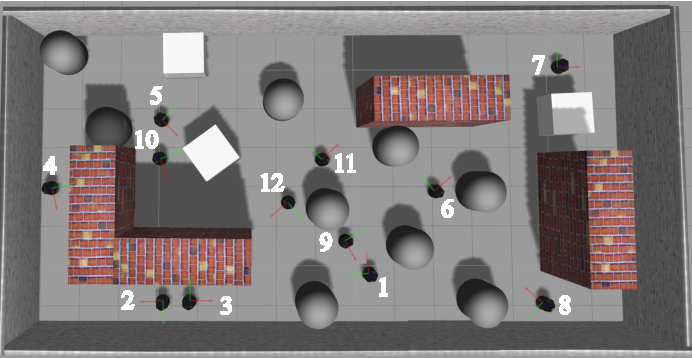
\includegraphics[width=0.8\columnwidth]{figure/obstacle_figs/start_env_number}
    \caption{The simulated indoor environment implemented in \textit{Gazebo} with various scenes and obstacles. The \textit{Turtlebot} is the experimental agent with a \textit{Kinect} camera mounted on it. One of the 12 locations marked in the figure is randomly set as the start point in each  training episode. The red arrow of every location represents the initial moving direction.}
   \label{fig:ob_environment_figure}
\end{figure}
%----------------------------------------------------


In our previous work \cite{tai2016deep}, the training datasets were collected in structured corridor environments. Depth images in these datasets were labelled with real-time moving commands from human decisions. In this chapter, to extend the navigation ability of the mobile robot, we set up a more complex indoor environment, as shown in Fig.~\ref{fig:ob_environment_figure}, in the \textit{Gazebo}\footnote{http://gazebosim.org} simulator. Besides the corridor-like traversable areas, there are much more complicated scenes like cylinders, sharp edges and multiple obstacles with different perceptive depths. These newly created scenes have never been used in the training of our previous supervised learning model \cite{tai2016deep}.

We use a \textit{Turtlebot} as the main agent in the simulated environment. A \textit{Kinect} RGBD camera is mounted on top of the robot. We can receive the real-time RGB-D raw image from the field of view (FOV) of the robot. All of the requested information and communications between agents are achieved through \textit{ROS}\footnote{http://www.ros.org} interfaces.



%----------------------------------------------------
\subsection{Deep Reinforcement Learning Implementation}
%-------------network structure---------------------
   \begin{figure}[!t]
      \centering
      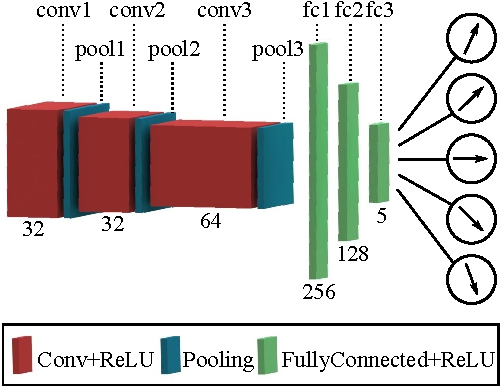
\includegraphics[width=0.75\columnwidth]{figure/obstacle_figs/cnn_structure}
      \caption{The network structure for the actor-evaluation estimation. It is a combination of convolutional networks for feature extraction and fullyconnected layers for policy learning. They have been separately proven to be effective in our previous works \cite{tai2016deep, tl_rcar_2016}.}
      \label{fig:ob_network_structure}
   \end{figure}
%-------------------------------------------------

As a standard reinforcement learning structure, we set the environment mentioned in Section \ref{sec:ob_simuenvi} as $e$. At each discrete time step, the agent selects an action $ a_t $ from the defined action set. In this section, the action set consists of five moving commands, namely \textit{left, half-left, straight, half-right} and \textit{right}. Detailed assignments of speeds related to the moving commands are introduced in Section \ref{sec:ob_experiment}. The only perception by the robot is the depth image $x_t$ taken from the \textit{kinect} camera after every execution of the action. Unlike in Atari games, where the reward $r_t$ is the change of the game's score, the only feedback used as the reward is a binary state, indicating whether a collision occurs or not. This is decided by checking the minimum distance $l_t$ through the depth image taken by the \textit{Kinect} camera. Once a collision occurs, we set a negative reward of $t_{ter}$ to represent the termination. Conversely,
we grant a positive reward of $t_{move}$ to encourage collision-free movement.

The state sequences $s_t$ in the simulated environment are regarded as a \textit{Markov Decision Process} (MDP) which is an alternate combination of moving commands and depth-image states, where $s_t = \{x_1,a_1,x_2,a_2,\dots, a_{t-1},x_t\}$. The sequence terminates once the collision happens. As the assumption of the MDP, $x_{t+1}$ is completely decided by $(x_t, a_t)$ without any reference to the former states or actions in $s_t$. The sum of the future rewards until the termination is $R_t$. With a discount factor $\gamma$ for future rewards, the sum of future estimated rewards is $R_t = \sum_{t'=t}^{T} \gamma^{t'-t} r_{t'}$, where $T$ means the termination time-step. The target of reinforcement learning is to find the optimal strategy $\pi$ for the action decision through maximizing the action-value function $Q^*(x,a) = max_{\pi}\mathbb{E}[R_t|x_t=x,a_t=a,\pi]$.
The essential assumption in DQN \cite{mnih2015human} is the \textit{Bellman equation}, which transfers the target to maximize the value of $r+\gamma Q^{*}(x',a')$ as
\[ Q^{*}(x,a)=\mathbb{E}_{{x'}\sim{e}}[r+\gamma \max \limits_{a'}Q^{*}(x',a')|x,a]. \]
Here, $x'$ is the state after acting action $a$ in state $x$.
DQN estimates the action-value equation by CNN with weights $\theta$, so that $Q(s,a,\theta) \approx Q^{*}(s,a)$.
%----------------------------algorithm-----------------------
\begin{algorithm}[!ht]
    \caption{Deep reinforcement learning algorithm}
    \label{alg:training_al}
    \begin{algorithmic}[1]
    \STATE {Initialize the weights of evaluation networks as $\theta^-$\\
           Initialize the memory $D$ to store experience replay\\
           Set the collision distance threshold $l_s$
           }
    \FOR {episode $ = 1, M$}
    \STATE {Randomly set the \textit{Turtlebot} to a start position\\
            Get the minimum intensity of depth image as $l_t$\\
        \WHILE{$l_t>l_s$}
            \STATE { Capture the depth image $x_t$ }
            \STATE {With probability $\varepsilon$ select a random action $a_t$ \\
                    Otherwise select $ a_t =\mathrm{argmax}_a Q(x_t,a;\theta^-)$ \\}
            \STATE { Move with the selected moving command $a_t$\\
                    Update $l_{t}$ with new depth information\\
            \IF{$l_{t}<l_s$}
                \STATE{ $r_t =r_{ter}$ \\
                $x_{t+1} = Null$}
            \ELSE
                \STATE{ $ r_t = r_{move}$ \\
                Capture the new depth image $ x_{t+1}$}
            \ENDIF \\
            }
            \STATE{
            Store the transition $(x_t,a_t,r_t,x_{t+1})$ in $D$} \\
            Select a batch of transitions  $(x_k, a_k, r_k, x_{k+1})$  randomly from $D$ \\
                \IF {$r_k = r_{ter}  $}
                    \STATE{ $y_k = r_k$   }
                \ELSE
                \STATE{  $ y_k = r_k+\gamma \max_{a'} Q(x_{k+1},a';\theta^-) $ }
                \ENDIF \\
           Update $\theta$ through a gradient descent procedure on the batch of $ (y_k - Q(\phi_k,a_k;\theta^-))^2$
        \ENDWHILE}
    \ENDFOR
\end{algorithmic}
\end{algorithm}
%-------------------------------------------------------

In this section, we use three convolutional layers for feature extractions of the depth image and use an additional three fullyconnected layers for obstacle avoidance learning. The structure is depicted as red and green cubes in Fig.~\ref{fig:network_structure}. To increase the non-linearity for better data fitting, each Convolutional or Fullyconnected layer is followed by a Rectified Linear Unit (ReLU) activation function layer.
The number under each Conv+ReLU or FullyConnected+ReLU cube is the number of channels of the output data related to this cube. The network takes one depth raw image as the input. The five channels of the final fully-connected layer \textit{fc3} are the values of the five moving commands. Also, to avoid the overfitting in the training procedure, both of the first two fully-connected layers \textit{fc1} and \textit{fc2} are followed with a dropout layer. Note that dropout layers are eliminated in the test procedure \cite{srivastava2014dropout}.

Algorithm \ref{alg:training_al} shows the workflow of our revised deep reinforcement learning process. Similar to \cite{mnih2015human}, we use the memory replay method and the $\varepsilon$-greedy training strategy to control the dynamic distribution of training samples. After the initialization of the weights for the convolutional networks shown in Fig.~\ref{fig:network_structure}, we set a distance threshold $l_s$ to check if the \textit{Turtlebot} collides with any obstacles. At the beginning of every episode, the \textit{Turtlebot} is randomly set to a start point among the 12 pre-defined start points shown in Fig.~\ref{fig:ob_environment_figure}.
This extends the randomization of the \textit{Turtlebot} locations from the whole simulation world and keeps the diversity of the data distribution saved in memory replay for training.

For the update of weights $\theta$, $y_k$ is the target for the evaluation network. It is calculated by summing the instant reward and the future expectation estimated by the networks with the former weights, as mentioned before in the \textit{Bellman equation}. If the sampled transition is a collision sample, the evaluation for this $(x_k , a_k)$ pair is directly set as the termination reward $r_{ter}$. Setting the training batch size to be $n$, the loss function is
\[
L({\theta}_i) = \frac{1}{n} \sum_{k}^{n}[(y_k-Q(x_k,a_k;{\theta}_i))^2].
\]
After the estimation of $Q(x_k, a_k)$ and $\max_{a'} Q(x_{k+1},a')$ with the former $\theta^-$, the weights $\theta$ of the network will be updated through back-propagation and stochastic gradient descent.

%-------------------Experiment and Result--------------------
\section{Experiment}
\label{sec:ob_experiment}
\subsection{Training}
At the beginning of the training, convolutional layers are initialized by copying the weights trained in \cite{tai2016deep} for the same layer structure. A simple policy learning networks structure was also separately proved in \cite{tl_rcar_2016} with three moving commands as output.
%---------------------------------------
\begin{table}[!ht]
    \centering
    \caption{Training parameters and the related values.}
    \label{tab:ob_training_parameters}
    \begin{tabular}{l r}
    \hline
    Parameter  & Value\\
    \hline
    batch size&32\\
    replay memory size & 3000\\
    discount factor $\gamma$ & 0.85\\
    learning rate & 0.0000001\\
    gradient momentum & 0.99\\
    distance threshold  $l_s$ & 0.55\\
    negative reward  $t_{ter}$ & -100\\
    positive reward  $t_{move}$ & 1\\
    \hline
    \end{tabular}
\end{table}
%-----------------------------------------

Compared with the step-decreasing learning rate in the training of the supervised learning model \cite{tai2016deep}, here we use a much smaller fixed learning rate in the end-to-end training for the deep reinforcement learning model. As the only feedback to motivate the network convergence, the negative reward for the collision between the robot and obstacles must be very large, as in \cite{tl_rcar_2016}. The training parameters are shown in Table~\ref{tab:ob_training_parameters} in detail. All models are trained and tested with Caffe \cite{jia2014caffe} on a single NVIDIA GeForce GTX 690.
\begin{table}[!ht]
    \centering
    \caption{Speeds of different moving commands.}
    \label{tab:moving_commands}
    \begin{tabular}{l  c c c c c c c c }
    \hline
        & &\multicolumn{5}{c}{ angular velocity (rad/s) }  & &line velocity  \\
  %  \hline
       & & Left & H-Left & Straight & H-right & Right& & (m/s) \\
    \hline
    Train & & 1.4 & 0.7&0 & -0.7& -1.4 & & 0.32\\
    \hline
    Test & &1.2& 0.6& 0& -0.6&-1.2 & &0.25\\
    \hline
    \end{tabular}
\end{table}
%---------------------------------------------

%-----------table of evaluation---------------
 \begin{table*}[!ht]
   \centering
   \caption{The average counts of moving steps and the average moving distances in every start point.}
   \label{tab:table_heatmapscore}
   \begin{tabular}{llp{0.5cm}p{0.5cm}p{0.5cm}p{0.5cm}p{0.5cm}p{0.5cm}p{0.5cm}p{0.5cm}p{0.5cm}p{0.5cm}p{0.5cm}p{0.5cm}}
   % \begin{tabular}{llp{0.5cm}p{0.5}p{0.5cm}ccccccccc}
   \hline
   &Model  & 1 & 2 & 3 & 4 & 5 & 6 & 7 & 8 & 9 & 10 & 11 & 12 \\
   \hline
   \multirow{6}{*}{Count} & SL &$ 7.6 $ &$ 16.4 $ &$ 33.4 $ &$ 3.0 $ &$ 21.1 $ &$ 20.2 $ &$ 6.9 $ &$ 14.0 $ &$ 16.7 $ &$ 5.6 $ &$ 10.6 $ &$ 19.6 $\\
   & RL  &$ 16.7 $ &$ \mathbf{102} $ &$ 4.0 $ &$ 19.1 $ &$ 14.5 $ &$ 7.4 $ &$ 5.0 $ &$ 3.0 $ &$ 16.8 $ &$ 7.0 $ &$ 18.4 $ &$ 36.6 $\\
   & DRL 500 &$ 6.6 $ &$ 3.7 $ &$ 5.8 $ &$ 4.0 $ &$ 5.0 $ &$ 3.5 $ &$ 4.0 $ &$ 9.8 $ &$ 8.3 $ &$ 4.0 $ &$ 21.0 $ &$ 36.3 $\\
   & DRL 4000 &$ 16.2 $ &$ 13.7 $ &$ 28.7 $ &$ 26.2 $ &$ 26.2 $ &$ \mathbf{26.9} $ &$ 10.4 $ &$ 41.8 $ &$ 13.0 $ &$ 20.3 $ &$ 12.4 $ &$ 23.1 $\\
   & DRL 7500 &$ 44.3 $ &$ 38.0 $ &$ 16.4 $ &$ 31.1 $ &$ 23.4 $ &$ 23.2 $ &$ \mathbf{29.1} $ &$ 30.8 $ &$ 18.1 $ &$ 24.6 $ &$ 27.7 $ &$ 21.4 $ \\
   & DRL 40000 &$ \mathbf{136} $ &$ 71.9 $ & $ \mathbf{66.1} $ & $ \mathbf{152} $ &$ \mathbf{91.7} $ &$ 17.8 $ &  $14.3 $ &$ \mathbf{103} $ &$ \mathbf{158} $ &$ \mathbf{86.0} $ &$ \mathbf{102} $ &$ \mathbf{113} $\\
   \hline
   \multirow{6}{*}{Dist.} & SL &$ 1.1 $ &$ 2.1 $ &$ 7.3 $ &$ 0.2 $ &$ 3.8 $ &$ 6.1 $ &$ 0.8 $ &$ 2.6 $ &$ 2.6 $ &$ 0.5 $ &$ 1.6 $ &$ 3.2 $ \\
   & RL &$ 3.6 $ &$ 3.0 $ &$ 0.2 $ &$ 5.4 $ &$ 1.8 $ &$ 0.7 $ &$ 0.2 $ &$ 0.2 $ &$ 4.1 $ &$ 0.6 $ &$ 3.9 $ &$ 9.0 $\\
   & DRL 500 &$ 1.1 $ &$ 0.5 $ &$ 0.5 $ &$ 0.6 $ &$ 0.7 $ &$ 0.5 $ &$ 0.5 $ &$ 0.7 $ &$ 0.8 $ &$ 0.6 $ &$ 0.8 $ &$ 0.9 $\\
   & DRL 4000 &$ 7.5 $ &$ 4.4 $ &$ \mathbf{17.6} $ &$ 10.3 $ &$ \mathbf{15.8} $ &$ \mathbf{10.7} $ &$ 2.1 $ &$ 20.3 $ &$ 2.4 $ &$ 5.7 $ &$ 2.8 $ &$ 10.1 $\\
   & DRL 7500 &$ 11.0 $ &$ \mathbf{20.5} $ &$ 6.0 $ &$ 10.6 $ &$ 9.4 $ &$ 9.0 $ &$ \mathbf{15.3} $ &$ 12.8 $ &$ 4.1 $ &$ 8.3 $ &$ 5.5 $ &$ 7.4 $\\
   & DRL 40000 &$ \mathbf{39.5} $ &$ 18.6 $ &$ 14.3 $ &$ \mathbf{21.0} $ &$ 7.6 $ &$ 10.5 $ &$ 2.7 $ &$ \mathbf{50.2} $ &$ \mathbf{33.0} $ &$ \mathbf{67.1} $ &$ \mathbf{19.2} $ &$ \mathbf{39.9} $\\
   \hline
   \end{tabular}
\end{table*}
%----------------------------------------------------------
Table~\ref{tab:moving_commands} lists the assignments of speeds for the five output moving commands both in training and testing procedures. All of the training or testing commands have the same line velocity. The various moving directions are declared with different angular velocities. The speeds for the training procedure are a little larger than the speeds for testing. With a higher training speed, the robot is motivated to collide aggressively and there will be more samples with negative rewards in the replay memory. In the testing procedure, a small speed can keep the robot making decisions more frequently.

%-------------triaining loss figure---------------------
   \begin{figure}[!ht]
      \centering
      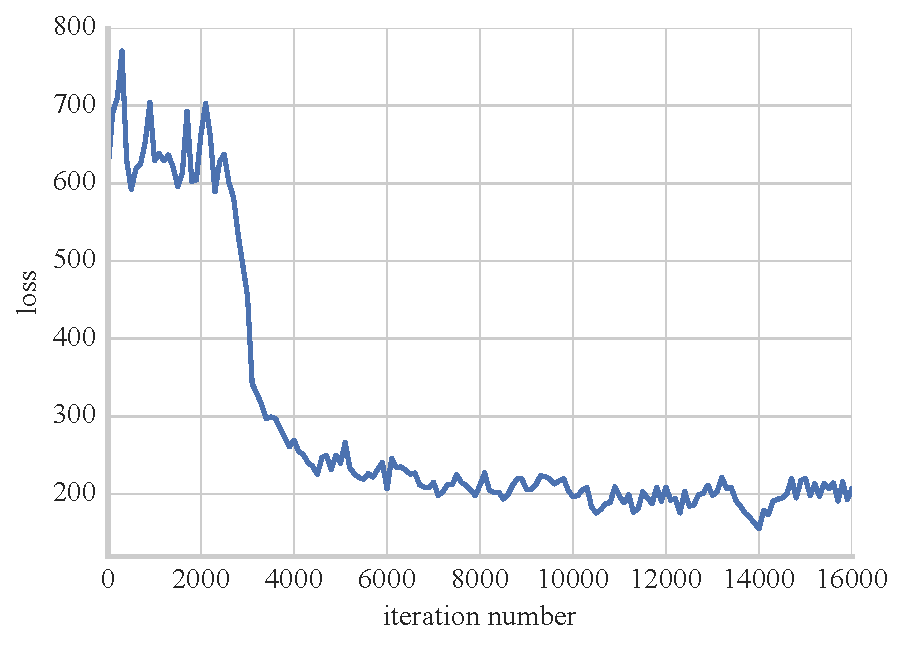
\includegraphics[width=0.8\columnwidth]{figure/obstacle_figs/loss_decrease}
      \caption{The loss decreasing curve as the training iterates. There is a batch of 32 samples used to do back-propagation in every iteration.}
      \label{fig:training_loss}
   \end{figure}
%----------------------------------------------------

Fig.~\ref{fig:training_loss} presents the loss reduction along training iterations. At each iteration, a batch including 32 depth images is randomly chosen from the replay memory. Unlike the training of conventional supervised learning methods, the loss of deep reinforcement learning may not converge to zero, depending extremely on the declaration of the negative reward. Among the estimation Q-values for state-action pairs, the maximum represents the optimal action. The value itself can limited present the sum of the future gains \cite{mnih2015human}. As seen in the figure, the loss converges after 4000 iterations. Test results of several trained models after 4000 iterations are compared in Section \ref{sec:analysis}.

\subsection{Analysis of Policy Tests} \label{sec:analysis}

%-----

We firstly look at the obstacle avoidance capability of the trained model. The trained DRL models after 500, 4000, 7500, and 40000 iterations are chosen to be tested in the simulated environment. The trained supervised learning (SL) model from \cite{tai2016deep} and the reinforcement learning (RL) model from \cite{tl_rcar_2016} are compared directly, without any revision of the model structure or tuning for the weights. In all 12 start points shown in Fig.~\ref{fig:ob_environment_figure}, every model starts ten episodes with the test speeds listed in Table~\ref{tab:moving_commands} for the five moving commands. Additionally, every test episode will stop automatically after 200 moving steps, so that the robot will not explore freely forever. With the same CNN structure for all the trained models, the forward prediction takes $48(\pm5)ms$ for each raw depth input.
After the forward calculation of the received real-time depth image, the robot chooses the moving command with the highest evaluation. The average counts of the moving steps for each start point are listed in Table~\ref{tab:table_heatmapscore}. The more moving steps, the longer the time the robot has been freely moving in the simulated environment without collision.
%---------------------------heatmap-----------------
\begin{figure*}[!ht]
    \centering
    \begin{subfigure}[t]{0.48\columnwidth}
      \centering
      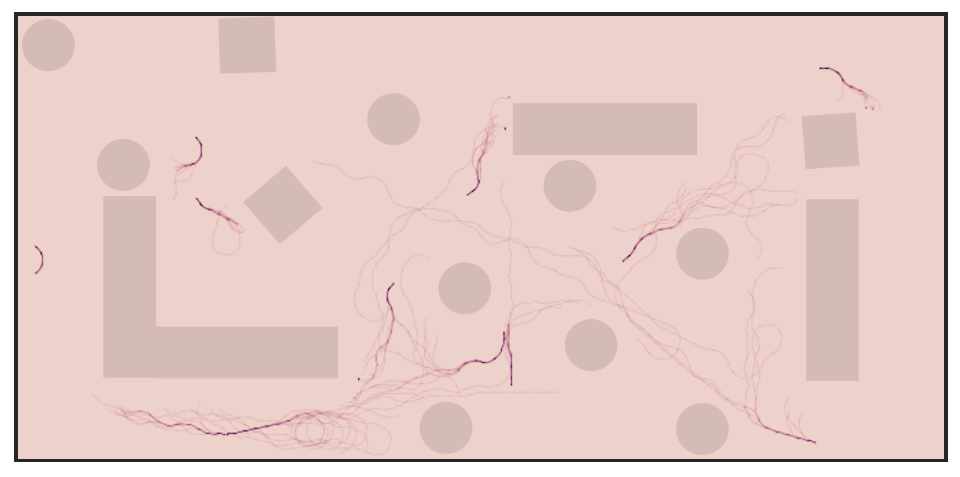
\includegraphics[width=\columnwidth]{obstacle_figs/locateheat/sl}
      \caption{Supervised Learning}
      \label{fig:heatsl}
    \end{subfigure}
    \begin{subfigure}[t]{0.48\columnwidth}
      \centering
      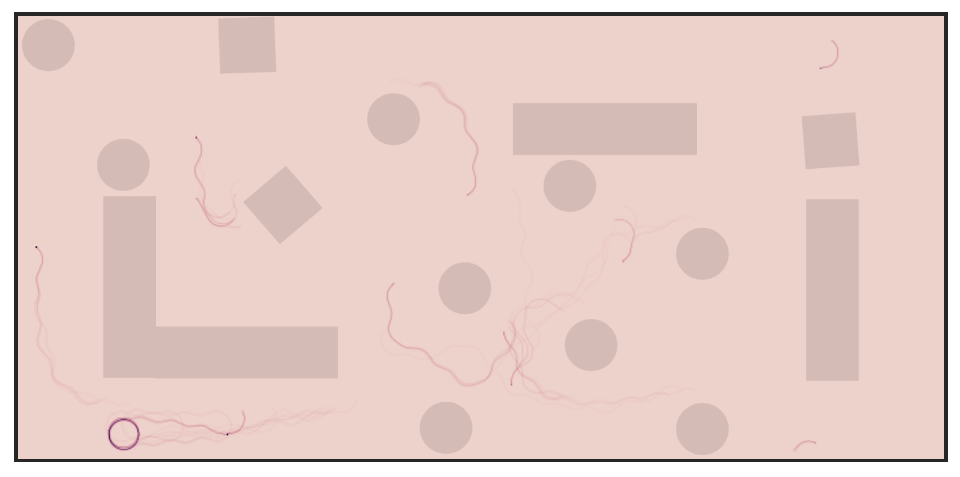
\includegraphics[width=\columnwidth]{obstacle_figs/locateheat/ql}
      \caption{Reinforcment Learning}
      \label{fig:heatql}
    \end{subfigure}
    \begin{subfigure}[t]{0.48\columnwidth}
      \centering
      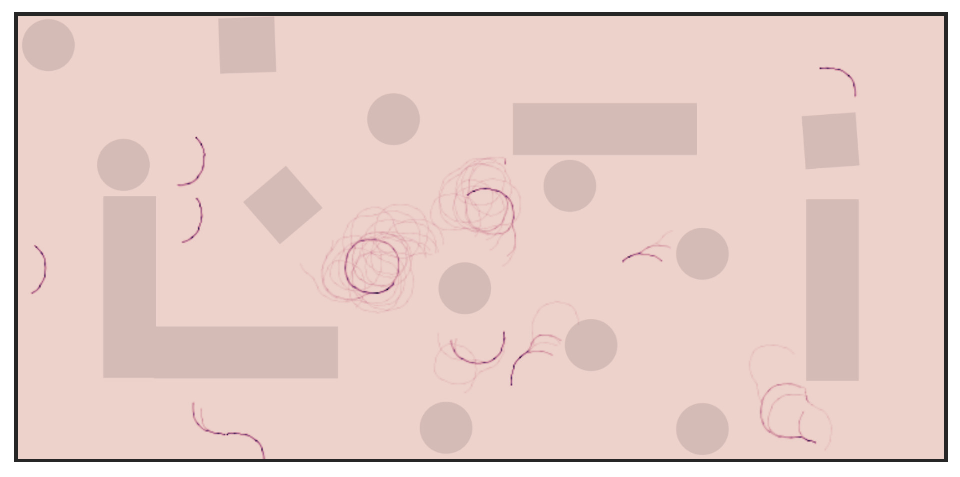
\includegraphics[width=\columnwidth]{obstacle_figs/locateheat/500}
      \caption{DRL 500 iterations}
      \label{fig:heat500}
    \end{subfigure}
    \begin{subfigure}[t]{0.48\columnwidth}
      \centering
      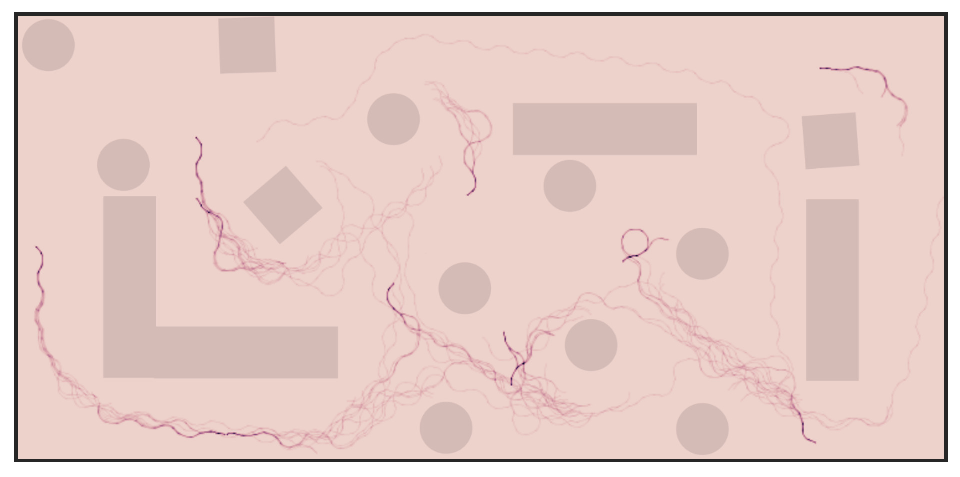
\includegraphics[width=\columnwidth]{obstacle_figs/locateheat/4000}
      \caption{DRL 4000 iterations}
      \label{fig:heat4000}
    \end{subfigure}
    \begin{subfigure}[t]{0.48\columnwidth}
      \centering
      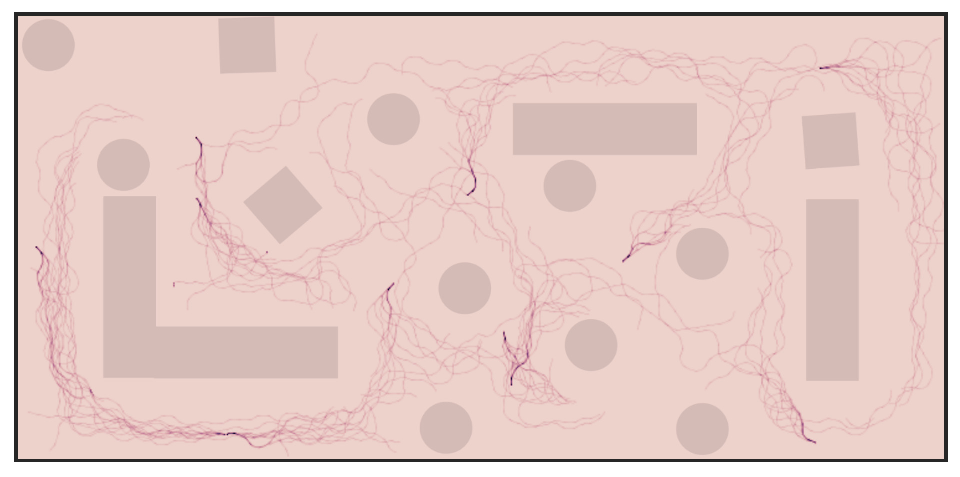
\includegraphics[width=\columnwidth]{obstacle_figs/locateheat/7500}
      \caption{DRL 7500 iterations}
      \label{fig:heat7500}
    \end{subfigure}
    \begin{subfigure}[t]{0.48\columnwidth}
      \centering
      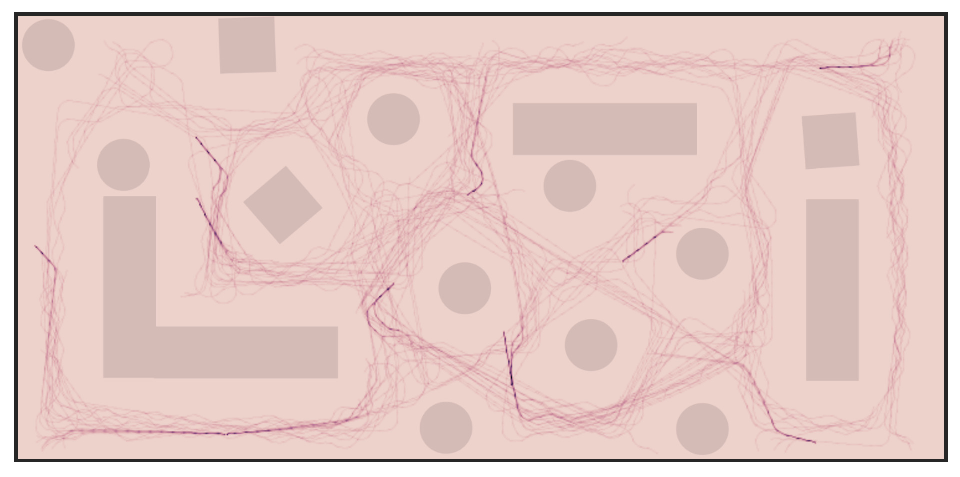
\includegraphics[width=\columnwidth]{obstacle_figs/locateheat/40000}
      \caption{DRL 40000 iterations}
      \label{fig:heat40000}
    \end{subfigure}
    \caption{Heatmaps of the trajectory points' locations in the 10 test episodes of each model for all 12 start points. The counts of points in every map grid are normalized to [0,1]. Note that the circles at the left-bottom corner of (b) and the middle of (c) are actually a stack of circular trajectories caused by the actual motion of the robot.}
    \label{fig:heat_map}
\end{figure*}
%---------------------------------------------------

The moving trajectory points of each model starting from all 12 positions are recorded. Fig.~\ref{fig:heat_map} depicts the trajectory after normalizing the counts of the trajectory points to $[0,1]$ in each map grid of the training environment. The trained model may choose the \textit{left} or \textit{right} command to rotate the robot in place so that no collisions will happen, as depicted in the circles in the left-bottom corner of Fig.~\ref{fig:heatql} and the middle of Fig.~\ref{fig:heat500}, for example. The very large moving count of the RL model in column 2 of Table~\ref{tab:table_heatmapscore} corresponds to the trajectory circle in Fig.~\ref{fig:heatql}. To avoid the appearance of this local minimum, the distances between the start and the endpoint are recorded as an additional evaluation metric. Note that, after a long exploration time, the robot may move back to the area near the start point. So the distance may not be perfectly equal to the obstacle avoidance ability of the trained model.

From the heat maps in Fig.~\ref{fig:heat_map}, we can see that the SL model cannot be adapted to the simulated environment, especially in the scenes with multiple obstacles at different depths and the RL model gives the worst of the results. In the training of the RL model \cite{tl_rcar_2016}, only the weights of the fully-connected network for policy iterations were updated iteratively. The DRL model shows significant improvement compared with the RL model because its training is end-to-end. Thus, not only is the policy network (\textit{fc} layers in Fig.~\ref{fig:network_structure}) developed for complicated scenes, but also the CNN model for feature representations.


Seen in Fig.~\ref{fig:heat_map}(c-f), the training for the obstacle avoidance ability of the DRL model is an online-learning process. In the 500-iteration case, the robot always chooses the same moving direction for any scenes. After 4000 iterations, it can be adapted to parts of the environment. However, In the 7500-iteration case, the robot can almost move freely in the whole simulated world. Furthermore, the robot usually chooses the optimal moving direction after 40000 iterations, like the more efficient trajectories in Fig.~\ref{fig:heat40000}. Unlike the fixed training datasets of the RL model, newly collected training samples of the DRL model are saved to replay memory increasingly. The evaluations of the training scenes are calculated by the current model, which is updated with the increasing number of training iterations. Thus, the robot obstacle avoidance ability will be increased over time.

The 40000-iteration case can almost thoroughly explore the trained environment. Considering the very long training time(12 hours) for 40000 iterations, we choose the model after 7500 iterations to do further analysis. The training time for 7500 iterations is 2.5 hours. This confirms that the mobile robot can be adapted to an unfamiliar environment by transferring the weights of the pre-trained SL model to the DRL framework with very short-term and end-to-end DRL training.

\subsection{Analysis of Receptive Fields in the Cognitive Process}

CNN models are usually considered to be black boxes and the internal activation mechanism of CNN is rarely analyzed. In \cite{zeiler2014visualizing}, the strongest activation areas of the feature representations are presented by backtracking the receptive field in the source input. We propose a backtracking method by multiplying the last layer of feature representations (\textit{pool3} in Fig.~\ref{fig:network_structure}) with a single channel convolutional filter.  The dimension of \textit{pool3} is $64 \times 20 \times 15 $ in this chapter. We multiply it with a convolutional kernel of size $1 \times 15 \times 15$, which is fixed with bilinear weights like the one used for upsampling of semantic segmentation in \cite{long2015fully}. After that, a $120 \times 160$ matrix of the same size as the input images.

\begin{table}[!ht]
    \centering
    \caption{Evaluations of moving commands for different scenes.}
    \label{tab:table_score}
    \begin{tabular}{ c c c c c c c c c}
    \hline
    \hline
      & & & & Left & H-Left & Straight & H-Right & Right \\
    \hline
     \multirow{2}{*}{S1} & & SL&  &$ 23.9 $ &$ \mathbf{26.3} $ &$ -10.6 $ &$ -35.3 $ &$ -34.4 $ \\
          &  &DRL& &$ \mathbf{-16.3} $ &$ -36.2 $ &$ -31.7 $ &$ -38.7 $ &$ -44.5 $ \\
    \hline
     \multirow{2}{*}{S2} & & SL &  &$ -18.2 $ &$ \mathbf{-0.1} $ &$ 46.2 $ &$ -30.1 $ &$ -8.8 $ \\
                 & &DRL& &$ -30.0 $ &$ -25.4 $ &$ -19.8 $ &$ -21.2 $ &$ \mathbf{-15.3} $\\
       \hline
    \multirow{2}{*}{S3} &  &SL&  &$ 4.2 $ &$ 5.9 $ &$ -21.3 $ &$ \mathbf{7.7} $ &$ -0.2 $ \\
                & &DRL& &$ \mathbf{-5.3} $ &$ -15.3 $ &$ -13.0 $ &$ -16.5 $ &$ -19.9 $ \\
       \hline
         \multirow{2}{*}{S4} & &SL&  &$ -4.0 $ &$ -5.5 $ &$ -15.2 $ &$ \mathbf{13.3} $ &$ -0.4 $ \\
                & &DRL& &$ -4.6 $ &$ -5.1 $ &$ \mathbf{-3.8} $ &$ -4.8 $ &$ -4.3 $ \\
     \hline
     \multirow{2}{*}{S5} & &SL&  &$ -17.4 $ &$ 12.3 $ &$ \mathbf{23.0} $ &$ -9.7 $ &$ -18.4 $ \\
            & &DRL& &$ \mathbf{-9.9} $ &$ -19.2 $ &$ -15.8 $ &$ -19.2 $ &$ -21.6 $ \\
    \hline
       \hline
     \multirow{2}{*}{R1} & &SL&  &$ -38.2 $ &$ 17.5 $ &$ \mathbf{27.4} $ &$ -15.6 $ &$ -1.9 $ \\
            & &DRL& &$ -84.1 $ &$ -89.3 $ &$ -71.8 $ &$ -78.8 $ &$ \mathbf{-63.2} $ \\
    \hline
     \multirow{2}{*}{R2} & &SL&  &$ -11.6 $ &$ \mathbf{45.6} $ &$ -50.3 $ &$ 4.1 $ &$ -8.3 $ \\
        & &DRL& &$ -8.3 $ &$ -9.3 $ &$ \mathbf{-7.1} $ &$ -8.6 $ &$ -7.5 $ \\
    \hline
     \multirow{2}{*}{R3} & & SL& &$ -18.4 $ &$ 32.2 $ &$ \mathbf{37.2} $ &$ -23.3 $ &$ -41.4 $ \\
        & &DRL& &$ \mathbf{-87.7} $ &$ -113.3 $ &$ -90.9 $ &$ -103.6 $ &$ -96.3 $ \\
       \hline
         \multirow{2}{*}{R4} & &SL& &$ 4.2 $ &$ 1.1 $ &$ -7.8 $ &$ -10.1 $ &$ \mathbf{15.2} $ \\
        & &DRL& &$ \mathbf{-87.6} $ &$ -141.1 $ &$ -115.2 $ &$ -134.8 $ &$ -137.4 $ \\
       \hline
         \multirow{2}{*}{R5}& &SL&  &$ 0.4 $ &$ -6.2 $ &$ -48.8 $ &$ \mathbf{32.8} $ &$ 11.9 $ \\
        & &DRL&    &$ -3.4 $ &$ -3.3 $ &$ \mathbf{-2.5} $ &$ -3.0 $ &$ -2.7 $ \\
    \hline
    \end{tabular}
\end{table}
%-------------------------------------------------------------------------------------------------

%-------------receptive real figure---------------------
\begin{figure*}[!ht]
    \centering
    \begin{subfigure}[t]{0.48\columnwidth}
      \centering
      \includegraphics[width=\columnwidth]{obstacle_figs/receptive/simurecpt}
      \caption{Simulation environmental samples}
      \label{fig:recep_simu}
    \end{subfigure}
    \begin{subfigure}[t]{0.48\columnwidth}
      \centering
      \includegraphics[width=\columnwidth]{obstacle_figs/receptive/simurecpt}
      \caption{Real-world samples}
      \label{fig:recep_real}
    \end{subfigure}
    \caption{The receptive fields of the feature representations extracted by CNN in both simulated environment samples and real-world samples. The purple area marked on the raw depth image represents the highest $10\%$ of activation values. Both the supervised learning model (SL) and the 7500-iteration deep reinforcement learning model (DRL) are compared. The arrow at the bottom of each receptive image is the chosen moving command based on evaluations listed in Table.~\ref{tab:table_score}. The left column shows the RGB images taken from the same scenes, for reference.}
    \label{fig:recep}
\end{figure*}
%----------------------------------------------------

We focus on the most substantial activation area of the receptive matrix. Fig.~\ref{fig:recep_simu} shows the highest $10\%$ of values of this matrix, marked on the related raw depth images in five specific simulated training samples. The receptive fields of the 7500-iteration DRL model are compared with those extracted from the SL model \cite{tai2016deep}. As mentioned above, these two models consist of the same convolutional structures. We choose five specific samples located in the fallible area based on the trajectory heat map of the SL model, as shown in Fig.~\ref{fig:heatsl}. Before being transported to the \textit{Softmax} layer, feature representations of the SL model were firstly transformed to five values related to the five commands in \cite{tai2016deep}. These values are listed with the action-evaluations estimated by the 7500-iteration DRL model in Table~\ref{tab:table_score}. For both of the models, the highest value corresponds to the optimal moving command.

%especially the untracked part
Note that the area beyond the detection range of the \textit{Kinect} camera is labelled as zero in the raw depth images. From Fig.~\ref{fig:recep_simu} and Table~\ref{tab:table_score}, for the SL model, the moving command towards the deepest area in the range receives the highest output value naturally. This motivates the convolutional model to activate the further area of the scenes, especially the junction with the untracked white fields. In \textit{S1}, the furthest reflection can help the robot avoid close obstacles. However, when there are multiple-level obstacles like in \textit{S2} and \textit{S3}, simply choosing the furthest part as the moving direction leads to collisions with nearby obstacles. Except for the furthest part, the DRL model also perceives the width of the route, both in the nearby area and the furthest area, as several horizontal cognitive stripes in the figure. That means the end-to-end deep reinforcement learning dramatically tunes the initial CNN weights from the SL model. From evaluations listed in Table~\ref{tab:table_score}, the DRL model not only helps the robot avoid instant obstacles, but also improves the traversable detection ability, like in \textit{S4} and \textit{S5}.
When the route in \textit{S4} is not wide enough to pass through, the DRL model chooses the fully turning moving command. However, the SL model always chooses the furthest area.

To prove the robustness of the trained model, five samples collected from a real-world environment by a \textit{Kinect} camera mounted on a real \textit{Turtlebot} are also tested, as shown in Fig.~\ref{fig:recep_real}. The related command evaluations for the SL model and the DRL model, as mentioned above, are listed in Table~\ref{tab:table_score} as well. Note that, these real-world scenes are not included in the training datasets for the SL model \cite{tai2016deep} either. The receptive fields of the SL model are still mainly focused on the furthest area. Output values in Table~\ref{tab:table_score} present the limited obstacle avoidance ability of the SL model for theses untrained samples. For the DRL model, even though only trained in the simulated environment, it keeps showing its ability to track the width of the route for real-world samples. In \textit{R1} and \textit{R2}, the trained DRL model successfully detects the traversable direction.
In \textit{R3}, it avoids the narrow space which is not wide enough to pass through. In \textit{R4}, it chooses the optimal moving direction to turn fully left. However, in \textit{R5}, when faced with irregular nearby obstacles which are not implemented in the training environment, it keeps tracking the width of the furthest area and fails to avoid irregular obstacles.

Another fact about the real-world tests is that the estimation of the action-value can reflect the future expectation to some extent. The estimation values of \textit{R3} and \textit{R4} listed in Table.~\ref{tab:table_score} for all moving commands are obviously less than the values of other scenes. This corresponds to the higher probability of collision when there are nearby obstacles.

%#######################################################
%-------------------Conclusion--------------------
\section{Conclusion}
\label{sec:ob_conclusion}
In this chapter, the utility of the deep reinforcement learning framework for robot obstacle avoidance is proved under end-to-end training.
The framework comprises two parts, convolutional neural networks for feature representations and fully-connected networks for decision making. We initialized the weights of the convolutional networks by a previously trained model based on our previous work \cite{tai2016deep}. The deep reinforcement learning model extends the cognitive ability of mobile robots for more complicated indoor environments in an efficient online-learning process continuously.
Analysis of receptive fields indicates the crucial promotion of end-to-end deep reinforcement learning: the feature representations extracted by convolutional networks are motivated substantially for the traversability of mobile robots both in simulated and real environments.





% this is try to set the conlusion as the same level as the PART in bookmark list.
\bookmarksetup{startatroot}
\addtocontents{toc}{\bigskip}
\chapter{Conclusion}
\label{ch:conclusion}

In this thesis, we have considered sensorimotor learning for ground robot navigation. We targeted to find an efficient pipeline to learn and deploy cognitive navigation policies in unstructured, unfamiliar, and dynamic environments.

% \section{Part \ref{part1}: From Supervised Learning to Reinforcement Learning}
To begin, we visualized the advantages of feature evolution for obstacle avoidance from supervised learning to deep reinforcement learning through extracting the receptive field of convolutional neural networks. The objective of this part was to discuss the necessity of deep reinforcement learning except the powerful supervised learning.

The model of the deep reinforcement learning was initialized from a pre-trained supervised model. We conducted the learning process in a simulated indoor environment. When deploying the pre-trained supervised learning model, it could not be adapted to the new environment, which was quite different from the training dataset. However, reinforcement learning kept updating its performance and adaptability for this new environment. What more interesting is the perceptive field of the trained network for different input depth images. The supervised learning model seemed to extract the edge with a higher gradient of depth information. However, the reinforcement learning model finally learned the width feature of the traversable area, which is more meaningful for obstacle avoidance.

In general, the results presented in this part of the thesis show the on-line learning ability of deep reinforcement learning. The learned feature can also generalize to unseen depth samples from the real world.

% \input{chapter/s5/part2}
% \input{chapter/s5/part3}
\section{Discussion and Outlook}
During this academic research, we have found more questions than answers in various fields. Currently, we have successfully applied model-free reinforcement learning and imitation learning in mobile robot navigation for both indoor and outdoor environments, considered the prediction and memory ability of neural networks and tackled the domain adaptation problem of the trained policy. However, there are still several less-addressed issues:
(1) The training of model-free reinforcement requires a large number of samples. Thousands of pieces of computation hardware and highly parallelised and distributed threads become necessary, especially for deep reinforcement learning \cite{barthmaron2018distributional, espeholt2018impala}. (2) Without implicitly or explicitly predicting the future states of the dynamic environment \cite{alahi2016social, chen2018crowd}, it is still challenging to generate an efficient navigation strategy among crowded pedestrians. And (3) Effective metrics to measure the visual-based autonomous driving in the real world is still missing.

Here, we briefly summarise the related future works for both deep reinforcement learning and imitation learning for navigation policies considering the two aforementioned issues.

For deep reinforcement learning, model-based algorithms are generally considered to be sample efficient \cite{deisenroth2013survey}. Predicting the forward image flow directly based on historical image states and actions was considered in \cite{finn2017deep}. They collected data through random motions of manipulators to estimate the visual-based dynamics model. This forward model was combined with model predictive control to finish several manipulation tasks. It can also be generalized to unknown objects.
Further, background occlusions \cite{ebert2017self} and registrations with start and target images \cite{ebert2018robustness} were considered to solve longer-moving and more complicated tasks.
Beyond leveraging the model with MPC, other research \cite{nagabandi2018neural} has let the model-free methods first imitate the behaviour of a model-based method. Combining model-free and model-based methods, TRPO \cite{schulman2015trust} was also improved with a learned dynamic model in \cite{kurutach2018model}. It yielded a much more stable learning process compared with the vanilla model-based reinforcement learning methods.
However, model-based reinforcement learning always lags behind the best model-free algorithms, especially when learning the model through high-dimensional approximators like deep neural networks. Employing uncertainty-aware dynamics models with sampling-based uncertainty propagation \cite{chua2018deep} has achieved comparable results to the best model-free algorithms on several challenging benchmark tasks. Extensions of model-based deep reinforcement learning on ground robot navigation would be exciting.

To predict the future state of nearby dynamic agents, learning a sensory-dynamics-model for autonomous driving is necessary. Considering the high dimension of RGB images, building this model on a top-view 3D lidar and first-person view semantic segmentation information through imitation learning may be a potential direction \cite{Rhinehart_2018_ECCV, rhinehart2018deep}.
% Semantics segmentation information should be enough to generate effective driving policy, and it can be naturally transferred to the real world \cite{pan2017virtual, yang2018eccv}.
% based on pre-trained semantic segmentation models \cite{he2017mask}.
Also, how to train a forward dynamics model efficiently with limited data is rarely considered. Xu \textit{et al.} \cite{xu2018algorithmic} introduced a novel algorithmic framework for model-based reinforcement learning algorithms with theoretical guarantees. This is particularly critical for mobile robot tasks. In terms of behaviour cloning, leveraging the implicit information but not just the raw sensor input may improve the efficiency of the model training. For example, gaze information has been proved to speed up the training of novice human learners.
Imposing this kind of information \cite{chen2019gaze, liu2019gaze} may also encourage the evolution of imitation learning for navigation.

In Part \ref{part3}, we have to measure the \textit{real-to-sim} pipeline for outdoor autonomous driving in another extreme simulated environment finally, because it is not trivial to achieve quantative results for this outdoor driving condition in the real world. An effective metric for the visual-based outdoor autonomous driving, especially for learning-based method, is still an open problem.



In general, research on sensorimotor learning is rapidly developing.
In this thesis, we explored the sensorimotor learning from both theoretical and practice perspectives and deployed various learning-based navigation policy from different sensors for the first time, in both indoor and outdoor environments and both real and simulated worlds.
To realize the target of \textit{living with robots} and allowing the robot to achieve \textit{human-like behavior}, sensorimotor learning will be expected to tackle various scenarios that we have not met before.


% \showthe\font
%%%%%%%%%%%%%%%%%%%%%%%%%%%%%%%%%%%%%%%%%%%%%%%%%%%%%%%%%%%%%%%%%%%%%%%%%
%                                                                       %
%      9) BIBLIOGRAPHY                                                  %
%                                                                       %
% This example uses bibtex to generate the required Bibliography. Refer %
% to the % the file ustthesis_test.bib for the entries of the           %
% Bibliography. Note that only the cited entries are printed.           %
%                                                                       %
% If BibTeX is not used to typeset the bibliography, replace the        %
% following line with the \begin{thebibliography} and \end{bibliography}%
% commands (the "thebibliography" environment) to process the           %
% Bibliography.                                                         %
%                                                                       %
%%%%%%%%%%%%%%%%%%%%%%%%%%%%%%%%%%%%%%%%%%%%%%%%%%%%%%%%%%%%%%%%%%%%%%%%%

%%%%%%%%%%%%%%%%%%%%%%%%%%%%%%%%%%%%%%%%%%%%%%%%%%%%%%%%%%%%%%%%%%%%%%%%%
%                                                                       %
% The recommended bibliography style is the IEEE bibliography style.    %
% "ustbib" defines the IEEE bibliography standard with the added        %
% ability of sorting the items by name of author.                       %
%                                                                       %
% If you are not using BibTeX to process your Bibliography, comment out %
% the following line.                                                   %
%                                                                       %
%%%%%%%%%%%%%%%%%%%%%%%%%%%%%%%%%%%%%%%%%%%%%%%%%%%%%%%%%%%%%%%%%%%%%%%%%

\bibliographystyle{plain}

\bibliography{ref}
% Please run "bibtex ustthesis_test" before the bibliography can be
% included.

%%%%%%%%%%%%%%%%%%%%%%%%%%%%%%%%%%%%%%%%%%%%%%%%%%%%%%%%%%%%%%%%%%%%%%%%%
%                                                                       %
%     10) APPENDIX (If Any)                                             %
%                                                                       %
%                                                                       %
%%%%%%%%%%%%%%%%%%%%%%%%%%%%%%%%%%%%%%%%%%%%%%%%%%%%%%%%%%%%%%%%%%%%%%%%%

\appendix

\chapter{LIST OF PUBLICATIONS}
\section*{Journal Publications}
\begin{enumerate}
	\item Jingwei Zhang*, {\bf Lei Tai}*, Peng Yun, Yufeng Xiong, Ming Liu, Joschka Boedecker, Wolfram Burgard, ``VR-Goggles for Robots: Real-to-sim Domain Adaptation for Visual Control", (* indicates equal contribution), \emph{IEEE Robotics and Automation Letters (RA-L)}, 2019.
  \item Peng Yun, {\bf Lei Tai}, Yuan Wang, Ming Liu, ``Focal Loss in 3D Object Detection", \emph{IEEE Robotics and Automation Letters (RA-L)}, 2019.
  \item {\bf Lei Tai}, Shaohua Li, Ming Liu, ``Autonomous Exploration of Mobile Robots through Deep Neural Networks", \emph{International Journal of Advanced Robotic Systems (IJARS)}, 2017.
  \item {\bf Lei Tai}, Ming Liu, ``Mobile Robots Exploration through CNN-based Reinforcement Learning", \emph{Robotics and Biomimetics}, 2016.
\end{enumerate}
\section*{Conference Publications}
\begin{enumerate}
	\item {\bf Lei Tai}, Peng Yun, Yuying Chen, Congcong Liu, Haoyang Ye, Ming Liu ``Visual-Based Autonomous Driving Deployment from a Stochastic and Uncertainty-Aware Perspective", \emph{IEEE/RSJ International Conference on Intelligent Robots and Systems (IROS)}, Macau, China, November 4-8, 2019.
	\item Yuying Chen*, Congcong Liu*, {\bf Lei Tai}, Ming Liu, Bertram Shi ``Gaze Training by Modulated Dropout Improves Imitation Learning", \emph{IEEE/RSJ International Conference on Intelligent Robots and Systems (IROS)}, Macau, China, November 4-8, 2019.
	\item Congcong Liu*, Yuying Chen*, {\bf Lei Tai}, Haoyang Ye, Ming Liu, Bertram Shi, ``A Gaze Model Improves Autonomous Driving", \emph{ACM Symposium on Eye Tracking Research \& Applications (ETRA)}, Denver, USA, June 25-28, 2019.
	\item {\bf Lei Tai}, Jingwei Zhang, Ming Liu, Wolfram Burgard, ``Socially-compliant Navigation through Raw Depth Inputs with Generative Adversarial Imitation Learning", \emph{International Conference on Robotics and Automation (ICRA)}, Brisbane, Australia, May 21-25, 2018.
	\item {\bf Lei Tai}, Giuseppe Paolo, and Ming Liu, ``Virtual-to-real Deep Reinforcement Learning: Continuous Control of Mobile Robots for Mapless Navigation, \emph{IEEE/RSJ International Conference on Intelligent Robots and Systems (IROS)}, Vancuver, Canada, September 24-28, 2017.
	\item {\bf Lei Tai}, Haoyang Ye, Qiong Ye, Ming Liu, ``PCA-aided Fully Convolutional Networks for Semantic Segmentation of Multi-channel fMRI", \emph{International Conference on Advanced Robotics (ICAR)}, Hong Kong, China, July 10-12, 2017.
  \item {\bf Lei Tai}, Shaohua Li, and Ming Liu, ``A Deep-Network Solution Towards Model-less Obstacle Avoidence", \emph{IEEE/RSJ International Conference on Intelligent Robots and Systems (IROS)}, Daejeon, Korea, October 9-14, 2016.
  \item {\bf Lei Tai}, Ming Liu, ``A Robot Exploration Strategy Based on Q-learning Network", \emph{IEEE International Conference on Real-time Computing and Robotics (RCAR)}, Angkor Wat, Cambodia, June 6-10, 2016.
\end{enumerate}
\section*{Workshop Publications}
\begin{enumerate}
	\item Congcong Liu*, Yuying Chen*, {\bf Lei Tai}, Ming Liu, Bertram Shi, ``Utilizing Eye Gaze to Enhance the Generalization of Imitation Network to Unseen Environments", \emph{International Conference on Machine Learning (ICML) Workshop}, June 14, Long Beach, USA, 2019.
	\item Oleksii Zhelo, Jingwei Zhang, {\bf Lei Tai}, Ming Liu, Wolfram Burgard, ``Curiosity-driven Exploration for Mapless Navigation with Deep Reinforcement Learning", \emph{International Conference on Robotics and Automation (ICRA) Workshop}, May 21, Brisbane, Australia, 2018.
\end{enumerate}
\section*{Technical Reports}
\begin{enumerate}
	\item {\bf Lei Tai}*, Jingwei Zhang*, Ming Liu, Joschka Boedecker, Wolfram Burgard, ``A Survey of Deep Network Solutions for Learning Control in Robotics: From Reinforcement to Imitation", (* indicates equal contribution).
	\item Jingwei Zhang, {\bf Lei Tai}, Joschka Boedecker, Wolfram Burgard, Ming Liu, ``Neural SLAM: Learning to Explore with External Memory".
	\item {\bf Lei Tai}, Ming Liu, ``Towards cognitive exploration through deep reinforcement learning for mobile robots".
\end{enumerate}


\endappendix



\end{document}
